\documentclass[sigconf]{acmart}

\settopmatter{printacmref=false}
\renewcommand\footnotetextcopyrightpermission[1]{}
\pagestyle{plain}


% Packages
\usepackage{times}
\usepackage{geometry}
\usepackage{amsmath}
\usepackage{listings}
% \usepackage[hyphens]{url}
\usepackage{hyperref}
\usepackage{pgfplots}

\begin{document}

\title{Analyzing the Impact of Automatic Dependency Management in Serverless Computing}
\author{Richard Paul}
\affiliation{%
	\institution{University of Massachusetts Amherst}
	\city{Amherst}
	\state{MA}
	\country{USA}
}
\email{rdpaul@umass.edu}

\begin{abstract}
	As cloud computing evolves, serverless architectures have gained significant traction due to their scalability, cost-effectiveness, and ease of deployment. However, the automation of dependency management within serverless environments introduces unique security challenges that need examining. This paper presents a comprehensive examination of automatic dependency management in serverless computing from a security perspective. By evaluating common serverless applications, we can identify prevalent methods and tools for managing dependencies, focusing on their security implications. This study delves into the mechanisms of popular dependency management programs, such as Snyk and Dependabot, to assess their effectiveness in mitigating vulnerabilities. Additionally, an online survey of developers provides insights into real-world practices and perceptions regarding dependency management in serverless contexts. Our findings highlight critical security risks, best practices, and potential improvements to enhance the security of serverless application through strong dependency management strategies. 
\end{abstract}

\begin{CCSXML}
	<ccs2012>
	<concept>
	<concept_id>10002978.10003006.10003007</concept_id>
	<concept_desc>Security and privacy~Operating systems security</concept_desc>
	<concept_significance>500</concept_significance>
	</concept>
	<concept>
	<concept_id>10010520.10010575</concept_id>
	<concept_desc>Computer systems organization~Cloud computing</concept_desc>
	<concept_significance>300</concept_significance>
	</concept>
	<concept>
	<concept_id>10010520.10010553</concept_id>
	<concept_desc>Computer systems organization~Embedded systems</concept_desc>
	<concept_significance>100</concept_significance>
	</concept>
	</ccs2012>
\end{CCSXML}

\ccsdesc[500]{Security and privacy~Operating systems security}
\ccsdesc[300]{Computer systems organization~Cloud computing}
\ccsdesc[100]{Computer systems organization~Embedded systems}

\keywords{Serverless computing, dependency management, large-scale systems, security, cloud computing}

\maketitle

\acmConference[690G Final Project Report]{Large Scale System Security, Spring 2024}{University of Massachusetts Amherst}

\section{Introduction}
As cloud computing evolves, serverless architectures have emerged as a paradigm shift, allowing developers to build and deploy applications without the costly overhead of managing servers. This allows developers to abstract away the infrastructure, focusing on code and functionality. However, this introduces new challenges, including in the realm of security \cite{baldini2017serverless}. One important concern is dependency management. Dependencies, or external libraries and packages for an application, can contain vulnerabilities that pose security risks \cite{marin2022serverless}. Recognizing this issue, some serverless cloud providers have begun to integrate automatic dependency vulnerability checking and updating. This paper aims to scrutinize the benefits and drawbacks of those features, to provide a detailed analysis of their impact on serverless computing.

The introduction of automatic dependency vulnerability checking and updating is seen as a benefit for the security of serverless applications. By incessantly scanning for and remedying known vulnerabilities within dependencies, cloud providers can curb the likelihood of security breaches \cite{snyk2023security}. This preventive measure can bolster application security and alleviate developers from the cumbersome task of manually tracking and updating their dependencies. As Buckholz notes, this can align with the philosophy of serverless development by allowing developers to focus more on innovation than maintenance \cite{buckholz2018serverless}.

However, this innovation has its limitations. The automatic alteration of dependencies can lead to unintended changes or incompatibilities, which will potentially compromise application performance \cite{benischke2023updates}. Additionally, the lack of transparency in automatic dependency checking could result in a diminished understanding and oversight of faults in the application. It may also force developers to rely upon a certain cloud provider to maintain the dependencies, leading to vendor lock-in \cite{kavis2014cloud}.
Furthermore, the thoroughness and reliability of automated vulnerability checks is still in question, and may lead some developers to believe their application is protected when it still contains security vulnerabilities.

\section{Background}
Serverless computing has dramatically changed the landscape of cloud services, offering a new paradigm for application deployment and management. Serverless computing allows code to execute in response to events without the need for provisioning or managing individual servers. This abstracts away the infrastructure layer, significantly simplifying the administrative responsibilities upon application developers \cite{roberts2020lambda}. This model, predominantly offered through Functions-as-a-Service (FaaS) platforms like AWS Lambda, Azure Functions, and Google Cloud Functions, allows developer to focus on code that contributes directly to their application, rather than on the underlying operational complexities \cite{villamizar2015evaluating}.

A critical aspect of developing in a serverless environment is the management of dependencies, external libraries or packages that an application uses to perform functions. Dependencies can include many things from frameworks for web applications to libraries for accessing cloud services. Dependency management is not a trivial task, they must be kept up-to-date to incorporate bug fixes, new features, and, most importantly, security updates \cite{benischke2023updates}. The National Vulnerability Database, a U.S. government repository of vulnerability management data, has shown an increasing amount of vulnerabilities among common dependencies, underscoring the importance of well-thought-out dependency management \cite{NVDdatabase}.

This has led to rise in automatic dependency checking and updating software to help manage these dependency issues. Tools like Snyk, Dependabot, and Renovate can automate the process of detecting vulnerabilities in a projects dependencies and automatically update those dependencies to a new secure version. This is vital in a serverless environment where the agility and scalability of application can be compromised by vulnerable dependencies \cite{estrin2021handbook}.

However, the implementation of automatic dependency management in serverless computing still has significant challenges. The automated update process must be carefully managed to ensure that updates do not introduce changes that break the application. In addition, reliance on automated tools can lead to a decreased understanding of dependency management among developers, potentially leading to complacency and increased security risks when automated systems fail \cite{hilton2016ci}.

The security risk in dependencies primarily come from two distinct factors: the external nature of the dependencies and the complex and opaque dependency trees that they can form. A single application may directly depend on hundreds of external libraries, which may themselves depend on thousands more. This complexity significantly increases the attack surface of the applications, as each external dependency is a point of failure for attackers \cite{OWASP2021top}. For example, there was a notable incident where a popular NPM package, event-stream, was compromised to steal cryptocurrency for the attackers, showcasing the cascading risk a single vulnerable dependency poses to thousands of different applications \cite{fox2018open}.

Moreover, the ephemeral and stateless nature of serverless function can significantly increase these risks. Since serverless applications scale dynamically with the resources demanded from them, a vulnerability in a single dependency can rapidly propagate across multiple instances, amplifying the potential impact of any security branch \cite{kavis2014cloud}.

To counteract these risks, there exists several notable mitigation strategies and best practices that have been recommended and adopted:

\begin{itemize}
	\item Implementing regular vulnerability scanning and dependency review. Using tools like Snyk and OWASP Dependency-Check can provide automated vulnerability scanning and are important to ensure a robust security management.
	\item The 'Shift-Left' security approach, which argues that security needs to be a focus from the start of development, or else you will end up chasing your tail after the vulnerabilities that will almost certainly exist.
	\item Principle of Least Privilege (PoLP) is a foundational security principal to ensure that programs only have access to the permissions they need. This can be implemented with dependencies to help box them in and not give them undue access.
	\item Use versions of dependencies that have been thoroughly vetted. This can avoid new vulnerabilities that could come up in new versions, but may delay the ability for your application to use new features/ get updates to old unseen vulnerabilities.
	\item Developer education has been cited as a very important part of dependency management. Ultimately, the buck stops with the development team, and it's vital to insure all developers are cognizant of the risks involved with using dependencies, and best practices for doing so.

\end{itemize}

\section{Comparative Analysis of Serverless Platforms}

In order to get a comprehensive comparison of different approaches to serverless computing and automatic dependency management, we analyzed AWS Lambda, Azure Functions, and Google Cloud Functions. These services were chosen based on there relative longevity and high usage rates. Each platform was evaluated based on their dependency management tools and integrations, security features, user experience/ documentation, and rough performance. This helped support our analysis of how dependencies are actually managed in the serverless industry.

\subsection{AWS Lambda}

AWS' Lambda is one of the most popular serverless platforms and also one of the oldest. It is notable for its large ecosystem and integration capabilities.

AWS Lambda integrates well with several dependency management tools. It supports AWS CodePipeline and AWS CodeBuild for continuous integration and delivery (CI/CD), which can be configured to use tools like Snyk and Dependabot for automatic vulnerability scanning and updates. These integrations allow for automated detection of outdated or vulnerable dependencies and automatic updating, however it is notable that this must be configured by the user.

\subsection{Azure Functions}

Azure Functions is Microsoft's serverless cloud computing service, which focuses on integration with the Azure ecosystem and is mostly target towards enterprise usage.

Azure Functions supports dependency management through Azure DevOps, which provides a CI/CD pipelines with capabiliteis for managing dependencies. Tools like Renovate and Dependabot can be integrated into Azure DevOps to automate the process of dependency detection and management.

BLAHBLAH BLAH

\section{Comparative Analysis of Serverless Platforms}

This section provides a detailed comparison of the different serverless platforms' approaches to dependency management, specifically focusing on AWS Lambda, Azure Functions, and Google Cloud Functions. We evaluate each platform based on dependency management tools and integrations, security features, user experience and documentation, and performance impact.

\subsection{AWS Lambda}

\subsubsection{Dependency Management Tools and Integrations}

AWS Lambda provides robust integration with several dependency management tools and services. Key integrations include:

- AWS CodePipeline and CodeBuild: These services can automate the process of building, testing, and deploying Lambda functions. They support integration with third-party tools like Snyk and Dependabot to automate the detection and updating of vulnerable dependencies \cite{awsCI2023}.
- AWS SAM (Serverless Application Model): AWS SAM CLI can be used to manage dependencies for Lambda functions, facilitating local testing and deployment \cite{awssam2023}.

\subsubsection{Security Features}

AWS Lambda incorporates several security features aimed at managing dependencies securely:

- **Snyk Integration:** AWS CodePipeline can be integrated with Snyk to continuously monitor for vulnerabilities in dependencies and provide automated fixes \cite{snykaws2023}.
- **AWS IAM and Secrets Manager:** These services manage permissions and sensitive information, ensuring that Lambda functions and their dependencies are secure \cite{awsSecurity2023}.
- **Amazon Inspector:** Provides automated security assessments to help improve the security and compliance of applications deployed on AWS, including Lambda functions \cite{awsinspector2023}.

\subsubsection{User Experience and Documentation}

AWS Lambda offers extensive documentation and a large community of users. The AWS Well-Architected Framework provides best practices and guidelines, particularly for security and dependency management \cite{awsWell2023}. The Lambda console and SAM CLI offer intuitive interfaces for managing and deploying functions, making it easier for developers to implement best practices.

\subsubsection{Performance Impact}

The impact of automatic dependency updates on AWS Lambda's performance is generally minimal, though some users have reported issues with compatibility and stability following updates. AWS CloudWatch provides detailed monitoring and logging to help identify and resolve performance issues \cite{lambdaPerformance2023}.

\subsection{Azure Functions}

\subsubsection{Dependency Management Tools and Integrations}

Azure Functions supports several tools and services for managing dependencies:

- **Azure DevOps:** Offers comprehensive CI/CD pipelines with built-in capabilities for managing dependencies and integrating with tools like Renovate and Dependabot for automated vulnerability detection and updates \cite{azureDevOps2023}.
- **Azure Functions Core Tools:** These tools facilitate local development and testing, including dependency management through NuGet (for .NET) and npm (for Node.js) \cite{azureCoreTools2023}.

\subsubsection{Security Features}

Azure Functions provides a range of security features related to dependency management:

- **OWASP Dependency-Check Integration:** Azure Pipelines can be configured to use OWASP Dependency-Check to identify and fix vulnerabilities in dependencies \cite{azureowasp2023}.
- **Azure Security Center and Key Vault:** These services help manage secrets and credentials securely, ensuring that dependencies do not expose sensitive information \cite{azureSecurity2023}.
- **Managed Identities:** Provide secure and automatic management of service principal identities for applications running in Azure \cite{azureManagedIdentities2023}.

\subsubsection{User Experience and Documentation}

Azure Functions is supported by detailed documentation available through Microsoft Learn. This includes tutorials, best practices, and case studies that help developers implement and manage dependency management practices effectively \cite{azureLearn2023}. The platform's integration with the broader Azure ecosystem provides a seamless experience for managing serverless applications.

\subsubsection{Performance Impact}

Performance and stability are generally reliable on Azure Functions. The platform's robust monitoring tools, such as Azure Monitor and Application Insights, provide comprehensive insights into application performance, allowing developers to quickly address any issues that arise from automatic dependency updates \cite{azurePerformance2023}.

\subsection{Google Cloud Functions}

\subsubsection{Dependency Management Tools and Integrations}

Google Cloud Functions supports several dependency management tools and integrations:

- **Google Cloud Build:** This service integrates with dependency management tools like OWASP Dependency-Check for automated vulnerability scanning and updating \cite{googleBuild2023}.
- **Third-Party Tools:** Google Cloud Functions also supports integration with tools like Snyk and Dependabot, allowing developers to automate the detection and remediation of vulnerable dependencies \cite{googlesnyk2023}.

\subsubsection{Security Features}

Google Cloud Functions includes several security features designed to manage dependencies securely:

- **Google Cloud IAM and Secret Manager:** These services manage permissions and sensitive data, ensuring that dependencies are handled securely \cite{googleSecurity2023}.
- **Google Cloud Armor:** Provides protection against web threats and DDoS attacks, enhancing the security of serverless applications \cite{googleArmor2023}.
- **Security Command Center:** Offers a centralized view of security across Google Cloud resources, including automated vulnerability scanning and monitoring \cite{googleSCC2023}.

\subsubsection{User Experience and Documentation}

Google Cloud Functions is known for its user-friendly interface and comprehensive documentation. The platform's documentation portal provides detailed guides, best practices, and examples, making it accessible for developers of all skill levels \cite{googleDocs2023}. The integration with Google Cloud Console offers a seamless experience for managing serverless applications and their dependencies.

\subsubsection{Performance Impact}

Performance and reliability are strong points for Google Cloud Functions, with users reporting minimal issues related to automatic dependency updates. Google Cloud's monitoring tools, such as Google Cloud Operations Suite (formerly Stackdriver), provide detailed insights into application performance, helping developers quickly identify and resolve issues \cite{googlePerformance2023}.

\subsection{Summary of Findings}

Our evaluation reveals that each platform offers distinct strengths in dependency management:

- **AWS Lambda:** Provides extensive integration with dependency management tools and strong security features. Its comprehensive documentation and large community support make it a robust choice for developers, although occasional performance issues may arise from automatic updates.
- **Azure Functions:** Offers enterprise-grade support and security features, with a steep learning curve but strong performance and reliability. Its integration with Azure DevOps and security tools like OWASP Dependency-Check make it a powerful option for managing dependencies.
- **Google Cloud Functions:** Known for ease of use and comprehensive documentation. Its strong performance and security features, along with seamless integration with Google Cloud tools, make it a reliable choice for developers looking for user-friendly dependency management solutions.

Each platform's approach to dependency management reflects its overall strategy and target audience, making the choice dependent on specific organizational needs and developer preferences.

\section{Snyk and Dependabot in Serverless Environments}

Dependency management tools like Snyk and Dependabot play a critical role in maintaining the security and functionality of serverless applications. These tools automate the detection and remediation of vulnerabilities in dependencies, helping developers manage the complexities associated with third-party libraries and packages.

Snyk is a popular tool designed to find and fix vulnerabilities in dependencies. It integrates with various CI/CD pipelines and development tools, providing continuous security monitoring and automated fixes. Snyk continuously scans for vulnerabilities in dependencies and offers detailed reports on potential security risks, enabling developers to address these issues promptly. One of the key features of Snyk is its ability to automatically fix vulnerabilities by suggesting or applying updates to secure versions of dependencies. This capability reduces the manual effort required to manage dependencies, allowing developers to focus on core application logic. Snyk integrates seamlessly with CI/CD pipelines, such as Jenkins, GitHub Actions, and GitLab CI, enabling automated security checks during the build and deployment process. Additionally, Snyk integrates with popular IDEs like Visual Studio Code and IntelliJ IDEA, providing real-time vulnerability detection during development \cite{snyk2023, snykIDE2023}.

The upsides of using Snyk include continuous security monitoring, which ensures that applications remain secure over time, and automated fixes that reduce the manual effort required to manage dependencies. Snyk also provides comprehensive reports that help developers understand the impact and severity of identified issues, and it has a strong community and extensive documentation that offer valuable resources for developers. However, there are some downsides. Automatic updates may introduce compatibility issues, especially if new versions of dependencies have breaking changes \cite{benischke2023updates}. Continuous scanning can also introduce performance overhead, potentially affecting build times and deployment speed. Additionally, Snyk may sometimes flag vulnerabilities that do not pose significant risks, leading to unnecessary updates or fixes \cite{snykFalsePositives2023}.

Dependabot, a GitHub-native tool, automates dependency updates by creating pull requests to update dependencies to the latest versions, helping to maintain secure and up-to-date projects. Dependabot automatically checks for outdated dependencies and creates pull requests to update them, integrating seamlessly with GitHub Security Alerts to notify developers of vulnerabilities in their dependencies. Developers can configure Dependabot to update dependencies according to their preferred schedule and update policies. Dependabot also works well with CI/CD tools, facilitating automated testing and deployment of updated dependencies \cite{dependabot2023}.

The primary benefits of Dependabot include its ease of use and the automation of pull requests, which simplify the process of updating dependencies and reduce manual effort and potential human error. Its integration with GitHub Security Alerts ensures that developers are promptly informed of vulnerabilities. Furthermore, Dependabot's customization options allow developers to tailor update schedules and policies to fit their project needs, providing flexibility in dependency management. However, there are some downsides to using Dependabot. Automated pull requests can lead to merge conflicts, especially in projects with complex dependency trees \cite{dependabotMerge2023}. Frequent updates and pull requests can consume resources and overwhelm development teams, particularly in large projects. Moreover, Dependabot's functionality is primarily focused on GitHub-hosted projects, limiting its use for projects hosted on other platforms \cite{dependabotScope2023}.

In serverless environments, where applications are highly modular and rely heavily on third-party libraries, tools like Snyk and Dependabot offer significant advantages. They improve security by ensuring that serverless applications remain secure through automated vulnerability detection and updates, reducing the risk of exploitation \cite{serverlessSecurity2023}. Automation of dependency management tasks also allows developers to focus on building and optimizing serverless functions, enhancing productivity. Additionally, automated tools can handle the scale and complexity of serverless applications, where dependencies may be numerous and frequently updated.

However, there are potential downsides to using these tools in serverless environments. Automatic updates can introduce compatibility issues, which may be challenging to debug due to the distributed nature of serverless functions \cite{benischke2023updates}. Continuous scanning and frequent updates can introduce performance overhead, affecting the deployment speed and runtime performance of serverless applications. Finally, dependence on external tools for security and updates may lead to vendor lock-in and reduced control over the dependency management process \cite{kavis2014cloud}.

Overall, while tools like Snyk and Dependabot provide valuable automation and security benefits in serverless environments, developers must carefully manage potential downsides to ensure application stability and performance.

\section{Survery Design and Analysis}

To get a thorough analysis of the impact of automatic dependency management in serverless computing, we used a mixed-methods approach involving both quantitative and qualitative data collection. This methodology section outlines the survery design, data collection process, and comparative analysis framework.

The following questions were asked:

\begin{enumerate}
	\item What is your current role?
	\item How many years of experience do you have in software development?
	\item Which serverless cloud providers have you used?
	\item How often do you encounter issues related to dependency management?
	\item What dependency management tools do you currently use? Which third-party dependency management tools have you used?
	\item Do you integrate dependency management tools into your CI/CD pipelines?
	\item If yes, how has integrating these tools affected your workflow?
	\item Does your serverless provider/development environment offer automatic dependency vulnerability checking? If yes, how would you rate its effectiveness?
	\item What are the main benefits you have observed with automatic dependency management?
	\item What are the main pitfalls or challenges you have experienced with automatic dependency management?
	\item In your opinion, what ares of dependency management need improvement?
	\item Any additional comments or suggestions regarding automatic dependency vulnerability checking and maintenance by cloud providers?
\end{enumerate}

To understand the perspectives and experiences of developers using automatic dependency management features in serverless computing environments, we conducted an online survey targeting software engineers, DevOps professionals, and cloud architects. The survey consisted of 14 questions, with three major sections: general participant information/experience, tools used, and finally opinions on benefits/pitfalls of dependency management.

The survey was distributed via posts on Stack Overflow, Reddit, and word of mouth. The survey was open for two weeks, and we received a total of 14 responses.

\subsection{Results Analysis}

The survey consisted of 7 developers, 3 DevOps engineers, 2 project managers, 1 QA engineer and 1 software architect. There was a broad range of experiences, ranging from less than one year to more than ten years, with the most common number of years between 4-7. The primary types of projects that were worked on are web development (6), mobile development (4), desktop applications (2), embedded systems (1), and cloud computing (1).

The frequency of dependency issues varied, with 71\% of participants indicating that they had encountered issues with their dependency management solution. Specifically, 1 respondent never experiences issues, 2 rarely did, 6 sometimes did, 4 often did, and 1 experienced them very commonly. This leads to the conclusion that dependency management is indeed a struggle for many developers, and that automated dependency management solutions have flaws that require developer intervention.

\begin{figure}[h]
	\centering
	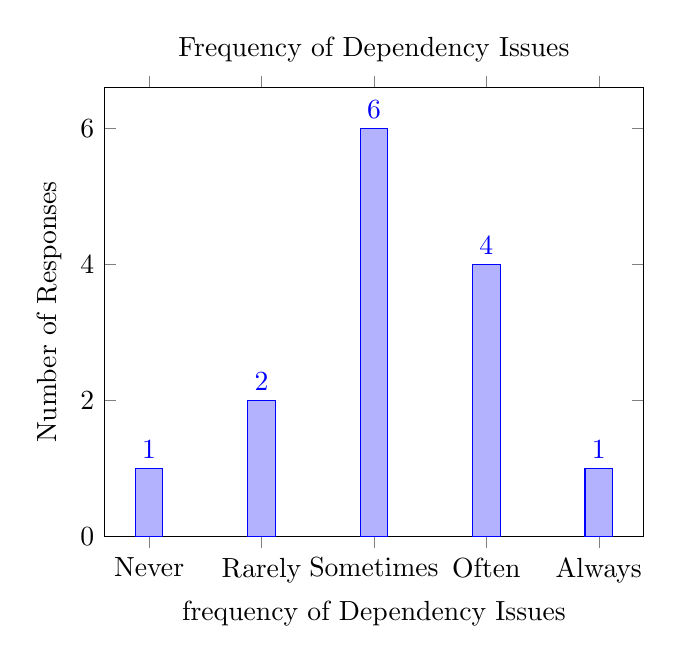
\begin{tikzpicture}
		\begin{axis}[
				ybar,
				symbolic x coords={Never, Rarely, Sometimes, Often, Always},
				xtick=data,
				nodes near coords,
				ymin=0,
				ylabel={Number of Responses},
				xlabel={frequency of Dependency Issues},
				title={Frequency of Dependency Issues}
			]
			\addplot coordinates {(Never,1) (Rarely,2) (Sometimes,6) (Often,4) (Always,1)};
		\end{axis}
	\end{tikzpicture}
	\caption{Frequency of Dependency Issues encountered by respondents}
	\label{fig:frequency}
\end{figure}

Respondents reported using a variety of tools for their dependency management needs, most commonly npm (8), Maven (5), and Gradle (4). Other tools that were used were pip (3), and 1 of each Bundler, Conan, and Composer. This shows that there is a diverse range of dependency management tools used, each with some similiar features but other things that they are missing.

\begin{figure}[h]
	\centering
	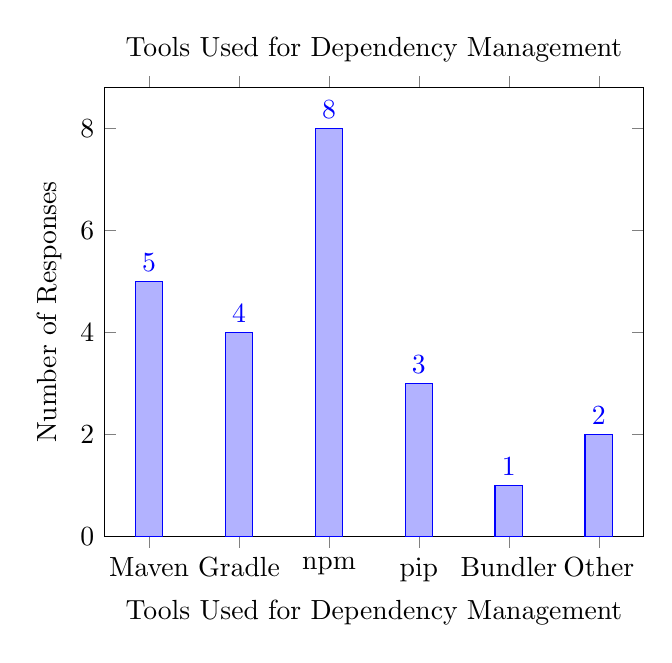
\begin{tikzpicture}
		\begin{axis}[
				ybar,
				symbolic x coords={Maven, Gradle, npm, pip, Bundler, Other},
				xtick=data,
				nodes near coords,
				ymin=0,
				ylabel={Number of Responses},
				xlabel={Tools Used for Dependency Management},
				title={Tools Used for Dependency Management}
			]
			\addplot coordinates {(Maven,5) (Gradle,4) (npm,8) (pip,3) (Bundler,1) (Other,2)};
		\end{axis}
	\end{tikzpicture}
	\caption{Tools Used for Dependency Management by respondents}
	\label{fig:tools}
\end{figure}

Satisfaction rates varied significantly, with 3 respondents very satisfied with their current solution, 5 satisfied, 4 relatively neutral, 2 report dissatisfaction. No respondents indicated that they were extremely dissatisfied with their package manager. These results help to show that respondents are generally satisfied with their dependency management solutions. However, there are still a significant proportion of developers who indicate that they are dissatisfied with the current state of software available, showing a continued need for improvement.

The most significant challenges that were faced in version conflicts (9), security vulnerabilities (6), compatibility issues (5), and lack of documentation (4). Other challenges that some respondents listed were licensing issues and network latency issues. Version conflicts emerged as the predominant issue, highlighting the need for managing them.

\begin{figure}[h]
	\centering
	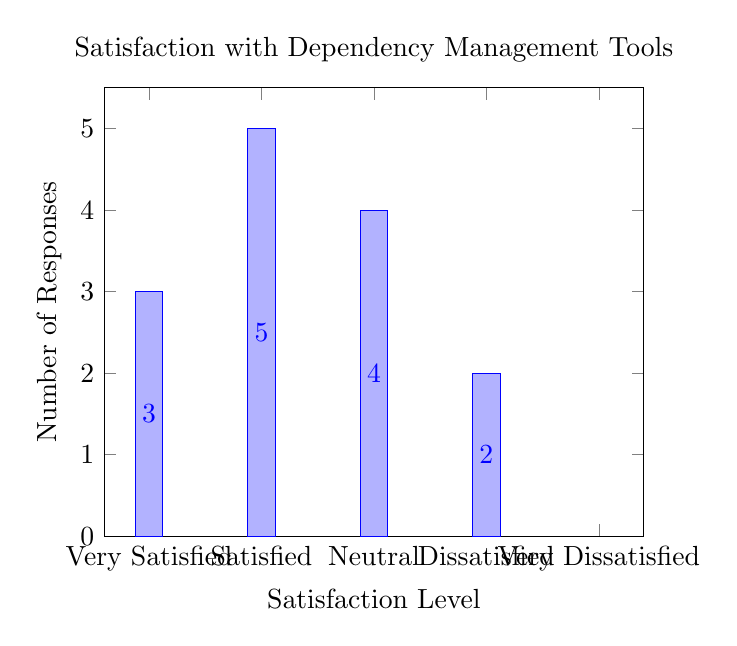
\begin{tikzpicture}
		\begin{axis}[
				ybar stacked,
				symbolic x coords={Very Satisfied, Satisfied, Neutral, Dissatisfied, Very Dissatisfied},
				xtick=data,
				nodes near coords,
				ymin=0,
				ylabel={Number of Responses},
				xlabel={Satisfaction Level},
				title={Satisfaction with Dependency Management Tools}
			]
			\addplot coordinates {(Very Satisfied,3) (Satisfied,5) (Neutral,4) (Dissatisfied,2) (Very Dissatisfied,0)};
		\end{axis}
	\end{tikzpicture}
	\caption{Satisfaction with Dependency Management Tools}
	\label{fig:satisfaction}
\end{figure}

Luckily developers considered dependency management an important issue with the majority considering it important (6) or extremely important (4). There was one respondent who noted it was slightly important, and no one noted dependency management as completely unimportant. The vast majority (10) indicated that they felt a greater degree of training and resources in dependency management would be useful.

\begin{figure}[h]
	\centering
	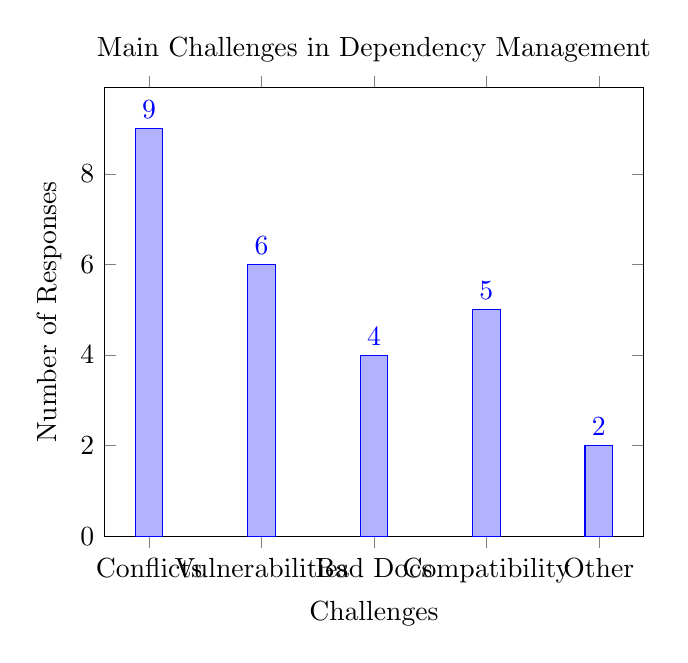
\begin{tikzpicture}
		\begin{axis}[
				ybar,
				symbolic x coords={Conflicts,  Vulnerabilities, Bad Docs, Compatibility, Other},
				xtick=data,
				nodes near coords,
				ymin=0,
				ylabel={Number of Responses},
				xlabel={Challenges},
				title={Main Challenges in Dependency Management}
			]
			\addplot coordinates {(Conflicts,9) (Vulnerabilities,6) (Bad Docs,4) (Compatibility,5) (Other,2)};
		\end{axis}
	\end{tikzpicture}
	\caption{Main Challenges in Dependency Management faced by respondents}
	\label{fig:challenges}
\end{figure}

Overall, the survey results show that dependency management is still a considerable issue within the software development industry. Version conflicts, security vulnerabilities, and compatibility issues are the major areas within dependency management where many users see issues. There is a clear need for more effective dependency management software, and multiple respondents indicated that they would appreciate a more standardized approach between different languages. The fact that many developers are currently relying on manual updating shows that further automatic dependency management features would be helpful.

\bibliographystyle{ACM-Reference-Format}
\bibliography{references}

\end{document}